\chapter{Detecția și izolarea defectelor}
\label{chap:detectie}
\section{Definirea defectelor}
Defectele sunt simulate modificând parametrul $C$ din ecuația emitter-ului \eqref{eq:emitter}. Modalitatea prin care se execută în cod simularea unui defect este prin apelarea metodei:

\lstinputlisting[language=Python, caption={Funcție pentru simularea defectelor},label={lst:set_emitter}, firstline=23,lastline=26]{\code/ENWrapper.py}

parametrii funcției $set\_emitter$ sunt:
\begin{itemize}
\item node\_inde - indexul nodului în care se simulează defectul
\item emitter\_val - magnitudinea defectului
\end{itemize}

Metoda mai întâi vefică dacă nodul cu indexul $node_index$ reprezintă doar o jonncțiune apoi setează magnitudinea defectului în nodul primit cu ajutorul funcției de bibliotecă $\mathbf{ENsetnodevalue}$ 

\section{Simulare dinamică pentru defecte în diferite noduri}

În continuare vom considera un scenariu de defect pentru rețea care constă în modificarea succesivă a parametrului de proporționalitate din relația de calcul a debitului de emitter \eqref{eq:emitter}. În imaginile următoare voi considera mai multe magnitudini de defect într-un anumit nod și voi reprezenta grafic răspunsul în timp al rețelei în același nod.

\begin{figure}[H]

\subfloat[Profile cu defect în nodul 14]{%
  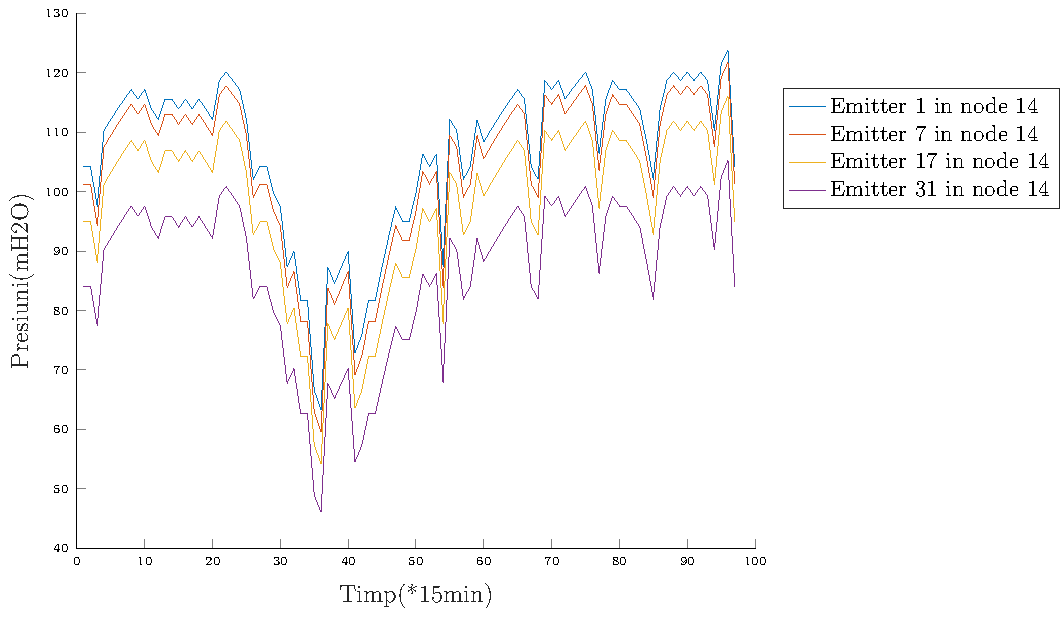
\includegraphics[width=0.5\textwidth]{\pics/c3_pics/emitter_node_same/emitter_node14}%
  \label{fig:emitter_node_same14}%
}\qquad
\subfloat[Profil cu defect în nodul 25]{%
  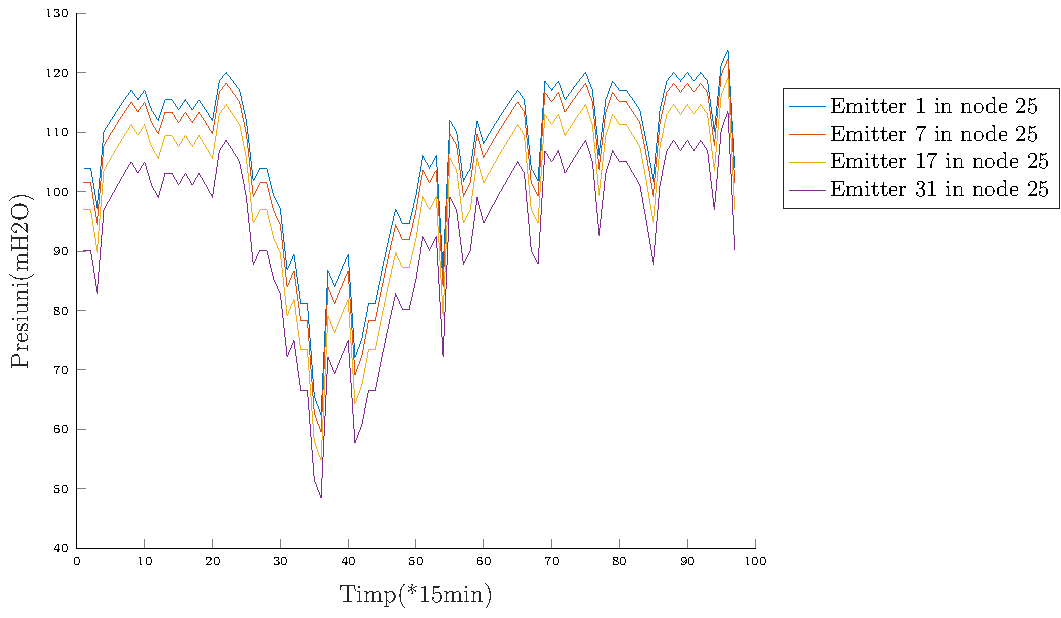
\includegraphics[width=0.5\textwidth]{\pics/c3_pics/emitter_node_same/emitter_node25}%
  \label{fig:emitter_node_same25}\qquad
}

\caption{Rezultate simulări defecte ușoare}
\label{fig:ref_emitter_soft}
\end{figure}

După cum se poate observa în imaginile \ref{fig:ref_emitter_soft} variația emitter-ului într-un nod produce în mod evident o modificarea a modului comun al caracteristicii $timp-presiune$. Din punctul de vedere al magnitudinolor de simulare pentru defecte, am considerat 2 clase de defecte, anume:
\begin{itemize}
\item defecte ușoare (soft faults) - cu valorile coeficientului de emitter mai mici de 35
\item defecte puternice (hard faults) - cu valorile emitter mai mari de 35 
\end{itemize}

Cele din urmă produc și modificări ale caracteristicii dinamice, introducând distorsiuni sau aplatizări ale mărimilor măsurate. Reprezentarea defectelor hard este reprezentată în figurile de mai jos:

\begin{figure}[H]

\subfloat[Profile cu defect puternic în nodul 14]{%
  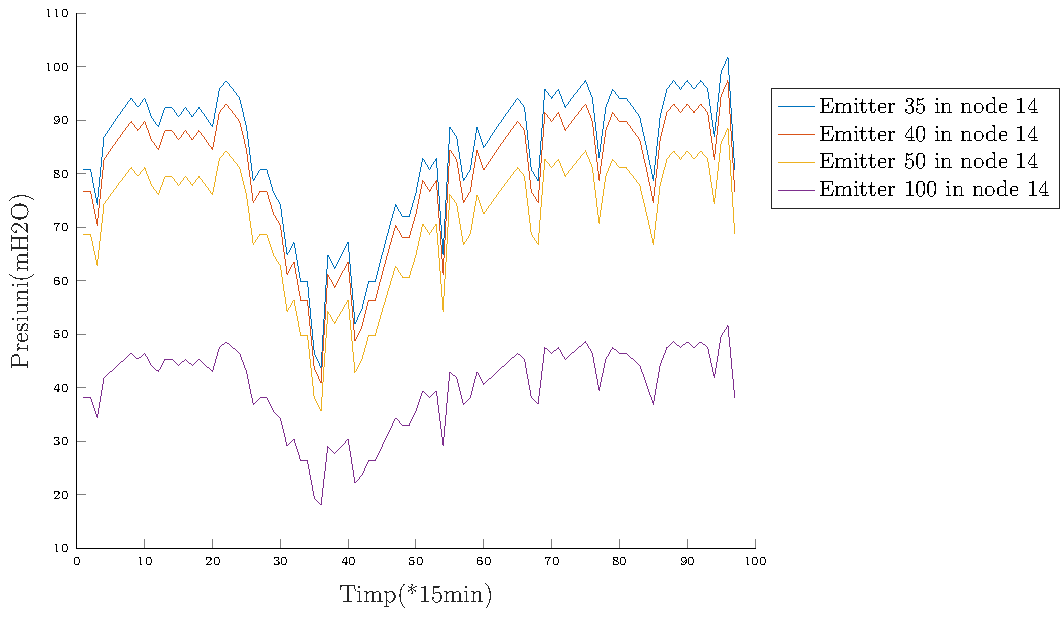
\includegraphics[width=0.5\textwidth]{\pics/c3_pics/emitter_node_same/emitter_hard_node14}%
  \label{fig:emitter_hard_node_same14}%
}\qquad
\subfloat[Profil cu defect puternic în nodul 25]{%
  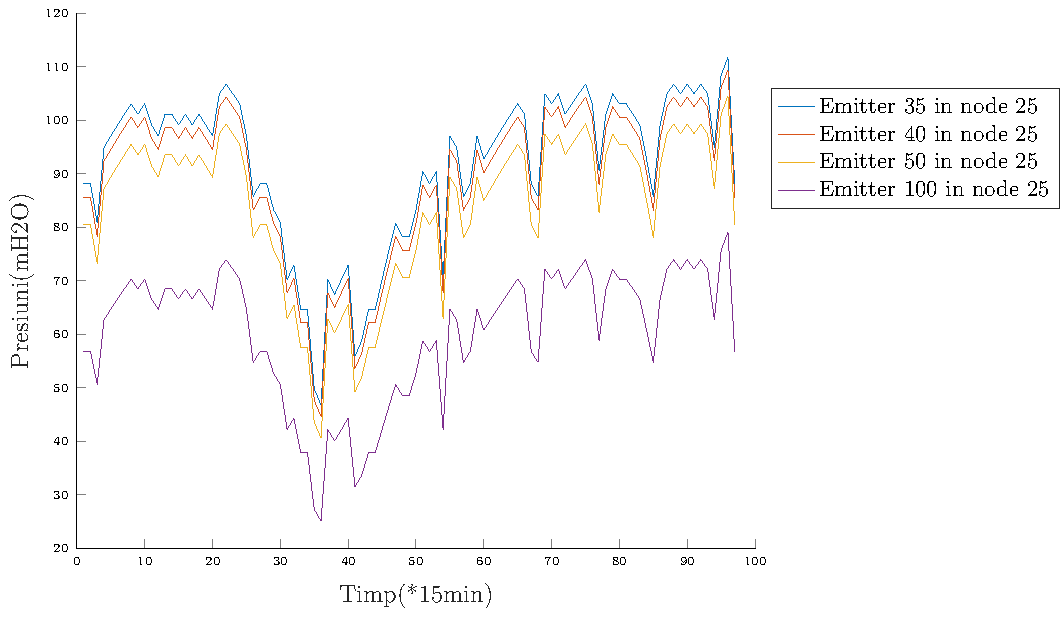
\includegraphics[width=0.5\textwidth]{\pics/c3_pics/emitter_node_same/emitter_hard_node25}%
  \label{fig:emitter_hard_node_same25}\qquad
}
\caption{Rezultate simulări defecte puternice}
\label{fig:ref_emitter_hard}
\end{figure}

Se observă de exemplu că pentru o valoare a emitter-ului de 100 caracteristica dinamică este deja modificată din cauza scurgerilor puternice din nod. 

Este relevantă împărțirea defectelor în mai multe clase de magnitudini pentru a putea valida un model de clasificare. Spre exemplu este normal să se întrebe dacă un model antrenat pe baza unui set date corespunzător unor magnitudini normale $C \in (0, 35)$ poate da rezultate semnificative pentru un set de date cu magnitudini ale emitter-ului puternice $C \geqslant 35$. 

\section{Preprocesarea datelor}
\label{sec:preproc}
În urma extragerii datelor din rețea este extrem de importantă etapa de prelucrare și preprocesare a datelor. Domeniul de preprocesare a datelor este unul extrem de vast și important în domeniul de învățare automată (engl. Machine Learning) și procesare de semnal. Preprocesarea datelor este etapa în care datele de intrare pentru un algoritm sunt aduse la o formă optimă pentru desfășurarea procesului impus, de exemplu în domeniul clasificării este important ca algoritmii să primească date care să fie scalate într-un anumit domeniu, pentru a asigura convergența\cite{dataPreprocessing}, \cite{GIGO}. Alegerea metodei de preprocesare este strâns legată de tipul de date disponibile și de starea acestora. În cazul rețelelor de apă, unde am ales caracteristica presiunii ca mărime de intrare pentru algoritm și ținând cont de răspunsul în timp al rețelei am considerat ca fiind necesare următoarele operații:

\begin{itemize}
\item eliminarea frontului comun și extragerea diferenței dintre semnalul nominal și cel măsurat în rețea
\item filtrarea semnalului obținut anterior
\end{itemize}

\section{Nomenclatura mărimilor alese}
\label{sec:nomenclatura}
Pentru a menține rigurozitatea și eleganța metodelor folosite este nevoie de o definire matematică pentru toate mărimile și metodele de filtrare folosite.

\subsection{Presiunea în regim dinamic}
Reprezintă o funcție de timp:
\begin{equation}
p_i : \mathbb{R} \longrightarrow \mathbb{R}^n, i \in V
\label{eq:press:func}
\end{equation}

unde $n$ reprezintă numărul de noduri al rețelei, iar $i$ reprezintă indexul nodului. 
Deoarece cazurile tratate în această lucrare reprezintă momente discrete de timp este important să definim presiunea măsurată în intervalele discrete în care este simulat procesul:
\begin{equation}
\mathbf{p}_i \in \mathbb{R}^{n \times p_{sim}}
\end{equation}

unde $p_{sim}$ reprezintă numărul de eșantioane pentru fiecare măsurătoare. Mergând mai departe în analiza simulării este de asemenea important să definim mărimea afectată de un defect în nodul $j$, de magnitudine $m$ și măsurată în nodul $i$:
\begin{equation}
\mathbf{p}^{j,m}_i \in \mathbb{R}^{n \times p_{sim}}
\end{equation}

Pentru cazul în care magnitudinea $m$ ia valori nule, atunci vom considera notația mărimii nominale:
\begin{equation}
\mathbf{p}^{j,0}_i = \mathbf{p}^{nom}_i, \forall j \in V
\end{equation}

Pentru valorile presiunii recoltate din rețea în nodul $i$ despre care nu se cunoaște nici o informație, vom considera notația
\begin{equation}
\widehat{\mathbf{p}}_i
\end{equation}

\subsection{Presiunea în regim static}
Considerând o plajă de momente de timp situate între indicii $rs_1 : rs_2$ unde se afla valorile de regim staționar ale procesului, putem defini o medie a regimului static în felul următor:
\begin{equation}
\overline{\mathbf{p}}_i^{j,m} = \frac{1}{rs_1 - rs_2 + 1} \sum_{k=rs_1}^{rs_2} \mathbf{p}_i^{j,m}[k] 
\label{eq:pmean}
\end{equation}

În aceeași manieră definim și media presiunii nominale în regim static:
\begin{equation}
\overline{\mathbf{p}}_i^{j,0} = \overline{\mathbf{p}_i}^{nom}, \forall j \in V
\label{eq:pmean_nom}
\end{equation}

Media presiunii măsurată în nodul $i$ și despre care nu se cunosc informații în legătură cu valoarea și poziția defectului:
\begin{equation}
\overline{\widehat{\mathbf{p}}}_i = \frac{1}{rs_1 - rs_2 + 1} \sum_{k=rs_1}^{rs_2} \widehat{\mathbf{p}}_i^[k] 
\label{eq:pmean_measured}
\end{equation}

\subsection{Reziduuri}
Așa cum a fost discutat în secțiunea \ref{sec:preproc}, preprocesarea datelor are un rol important iar în cazul analizei și clasificării defectelor în rețelele cu apă, este nevoie să definim caracteristica prelucrată care va fi folosită mai apoi în procesul de izolare a defectelor. Reziduul absolut reprezintă diferența dintre valoarea măsurată în rețea și valoarea nominală, aici putem discerne două cazuri:
Reziduu temporal:
\begin{equation}
\mathbf{r}_i^{j,m} = \mathbf{p}_i^{j,m} - \mathbf{p}_i^{nom}
\label{eq:temp_residual}
\end{equation}
Reziduu atemporal, calculat ca diferența dintre cele două valori mediate pe intervalul staționar al caracteristicii:
\begin{equation}
r_i^{j,m} = \overline{\mathbf{p}}_i^{j,m} - \overline{\mathbf{p}}_i^{nom}
\label{eq:absolute_residual}
\end{equation}

iar pentru valorile reziduului despre care nu se cunosc încă lucruri folosim notația din stilul anterior:
\begin{equation}
\widehat{r}_i = \overline{\widehat{\mathbf{p}}}_i - \overline{\mathbf{p}}_i^{nom}
\label{eq:measured_residual}
\end{equation}

Alte tipuri de reziduuri preprocesate sunt relative:
\begin{equation}
rrelativ_i^{j,m} = \frac{r_i^{j,m}}{\overline{\mathbf{p}}_i^{nom}} 
\label{eq:relative_residual}
\end{equation}

Reziduurile normate:
\begin{equation}
rnorm_{i}^{j,m} =  \frac{r_i^{j,m}}{ \norm{r_{1:n}^{j,m}}} 
\label{eq:norm_residual}
\end{equation}

Reziduurile scalate:
\begin{equation}
rscal_{i}^{j,m} = \frac{r_i^{j,m} - \min r_{1:n}^{j,m}}{ \max r_{1:n}^{j,m} -  \min r_{1:n}^{j,m}}
\label{eq:scaled_residual}
\end{equation}


Ca semnificație notațiile prezentate în \ref{sec:nomenclatura} care conțin simbolul~ $\widehat{}$~ fac referire la datele folosite pentru validarea modelului iar valorile unde se specifică nodul defectului și magnitudinea acestuia sunt considerate ca fiind date de antrenare și testare. Astfel în contextul definirii setului de dat pe care vom aplica algoritmii de calsificare va trebui să definim matricea:
\begin{equation}
\mathbf{R<tip>}^{j, m} \in \mathbb{R}^{n_{d} \times n}
\label{eq:residual_mat}
\end{equation}

Unde croșetele din formulă reprezintă un înlocuitor pentru metoda de reziduu folosită iar $n_{d}$ reprezintă numărul de defecte tratate în setul de date. De asemenea pentru fiecare linie a matricei \eqref{eq:residual_mat} putem defini perechea
\begin{equation}
\left( \mathbf{R}<tip>(d,:), y_{d} \right)
\label{eq:residual_label}
\end{equation} 
Unde $ \mathbf{R}<tip>(d,:)$ reprezintă răspunsul rețelei prin reziduuri la defectul $d$. Iar $y_{d}$ reprezintă eticheta pentru acest set de date, anume, nodul în care a avut loc defectul.

\section{Calcul și prezentare reziduuri}
În continuare vom prezenta grafic reziduurile temporale normalizate care apar în rețea pentru diferite scenarii ale defectelor definite anterior.
Astfel vom considera nodurile de măsurătoare ca o submulțime  a lui $V' \subset V$ și $ V = \{5, 11, 15, 17, 21, 27\}$, nodurile în care s-au simulat defecte sunt $V_{d} = \{11, 17, 27,29\}$.

 
\begin{figure}[H]
\begin{tabular}{cc}
\subfloat[Reziduuri pentru defect în nodul 11, magnitudine 29]{%
  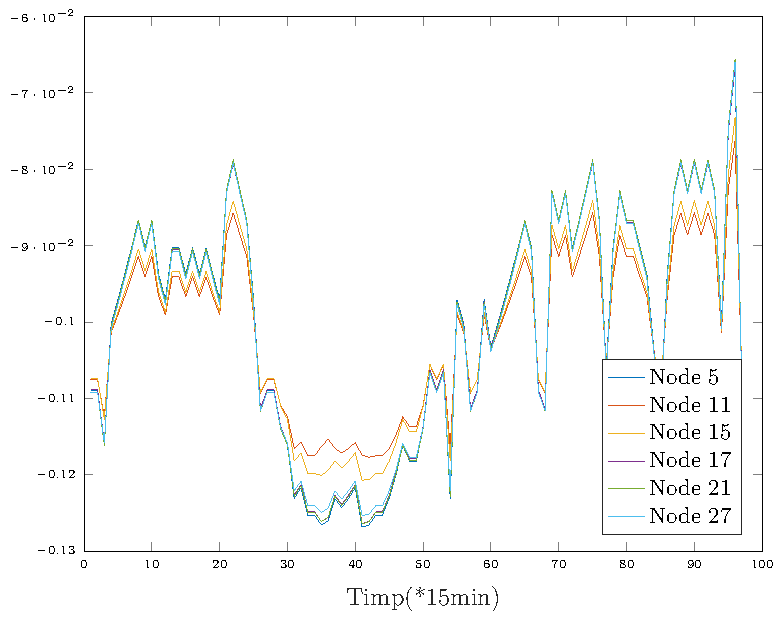
\includegraphics[width=0.5\textwidth]{\pics/c3_pics/residuals/time_res_emitter11_mag29}%
  \label{fig:residual_time_11}%
} &
\subfloat[Reziduuri pentru defect în nodul 17, magnitudine 29]{%
  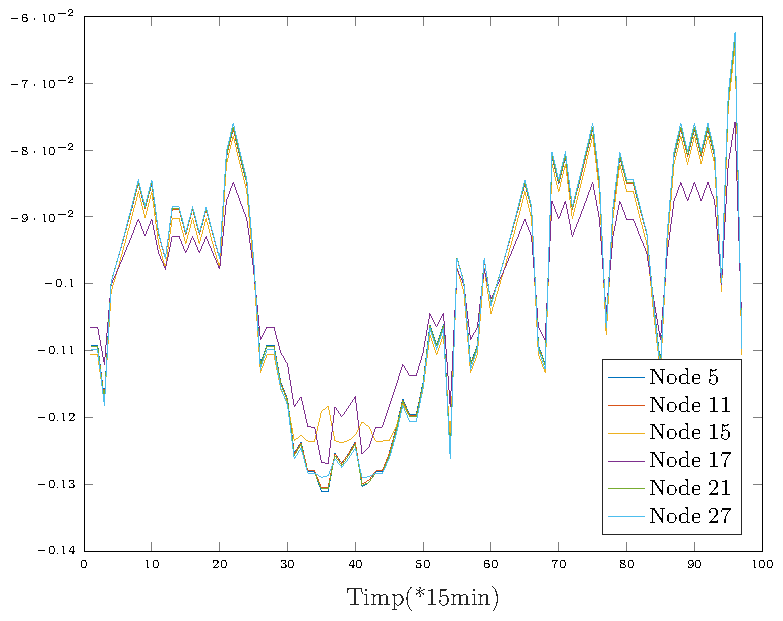
\includegraphics[width=0.5\textwidth]{\pics/c3_pics/residuals/time_res_emitter17_mag29}%
  \label{fig:residual_time_17}%
} \\

\subfloat[Reziduuri pentru defect în nodul 21, magnitudine 29]{%
  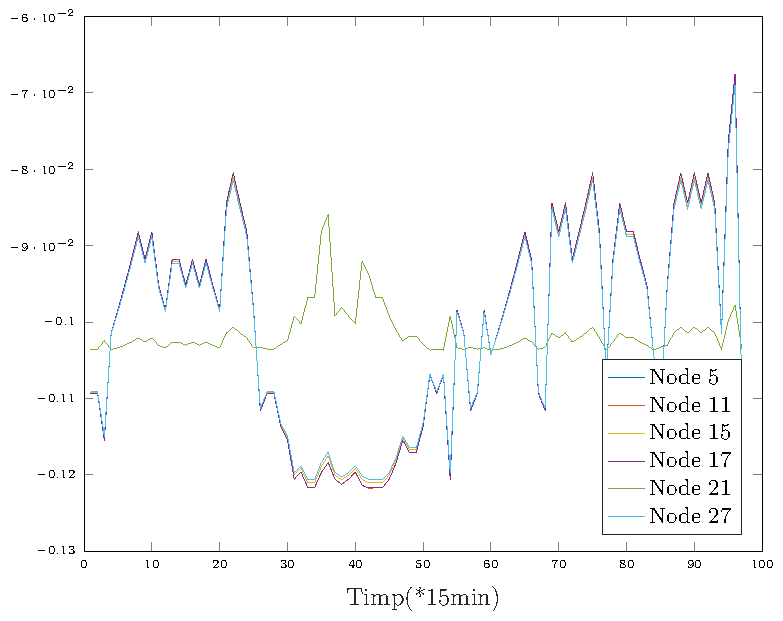
\includegraphics[width=0.5\textwidth]{\pics/c3_pics/residuals/time_res_emitter21_mag29}%
  \label{fig:residual_time_21}%
}&

\subfloat[Reziduuri pentru defect în nodul 27, magnitudine 29]{%
  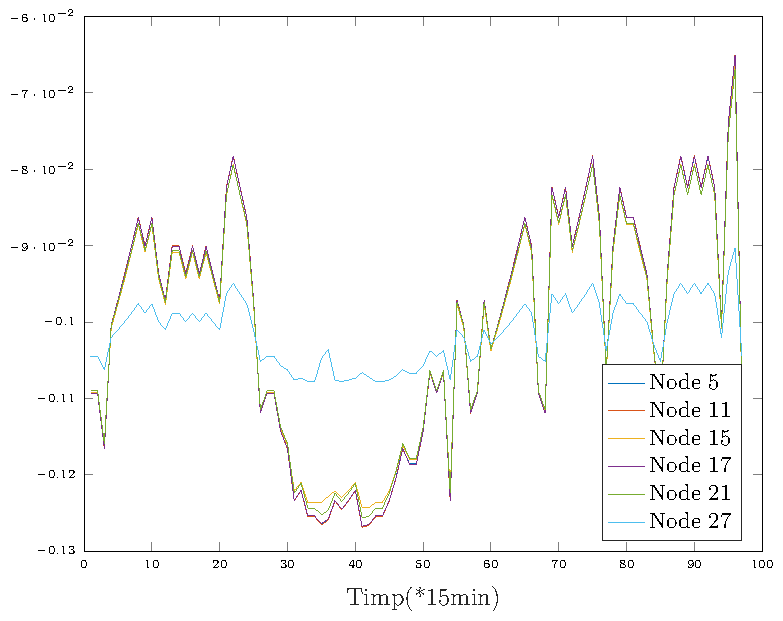
\includegraphics[width=0.5\textwidth]{\pics/c3_pics/residuals/time_res_emitter27_mag29}%
  \label{fig:residual_time_27}%
} 
\end{tabular}
\caption{Reziduuri rețea}
\label{fig:rez_time}
\end{figure}


Se poate observa că în figurile \ref{fig:rez_time} reziduul cel mai pronunțat ca funcție de timp se găsește în nodul în care se simulează și defectul - lucru natural și de așteptat. O caracteristică importantă a acestei rețele de apă este faptul că există o dependență între diferitele răspunsuri în timp ale caracteristicii de presiune, fapt care ne permite să exploatăm redundanțele din rețea și să prezicem cu o acuratețe relativ ridicată defectele.

Este necesar acum să prezentăm profilurile reziduurilor atemporale, care în final vor reprezenta caracteristicile de intrare pentru algoritmul de clasificare și selecție de senzori.

\begin{figure}[H]
\begin{tabular}{cc}
\subfloat[Reziduuri pentru defect în nodul 11, magnitudine 25]{%
  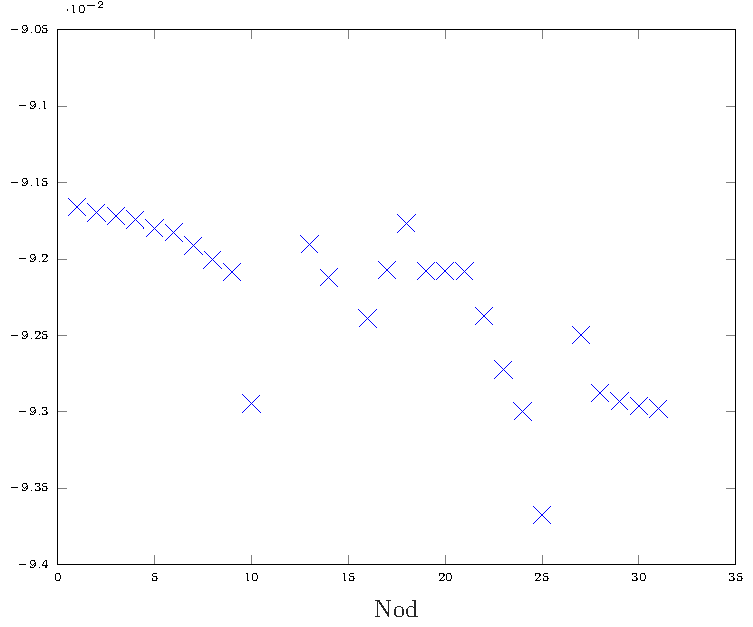
\includegraphics[width=0.5\textwidth]{\pics/c3_pics/residuals/atem_res_emitter11_mag25}%
  \label{fig:residual_atemp_11}%
} &
\subfloat[Reziduuri pentru defect în nodul 17, magnitudine 25]{%
  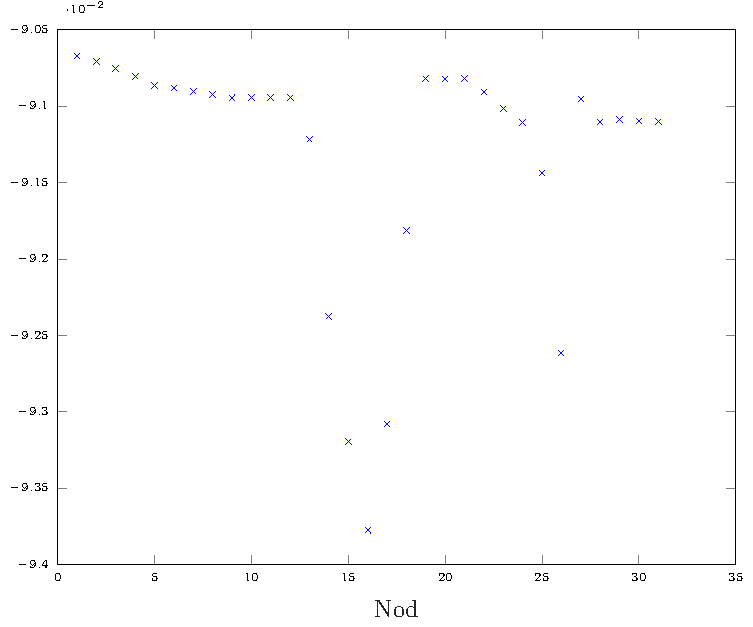
\includegraphics[width=0.5\textwidth]{\pics/c3_pics/residuals/atem_res_emitter17_mag25}%
  \label{fig:residual_atemp_17}%
} \\

\subfloat[Reziduuri pentru defect în nodul 21, magnitudine 25]{%
  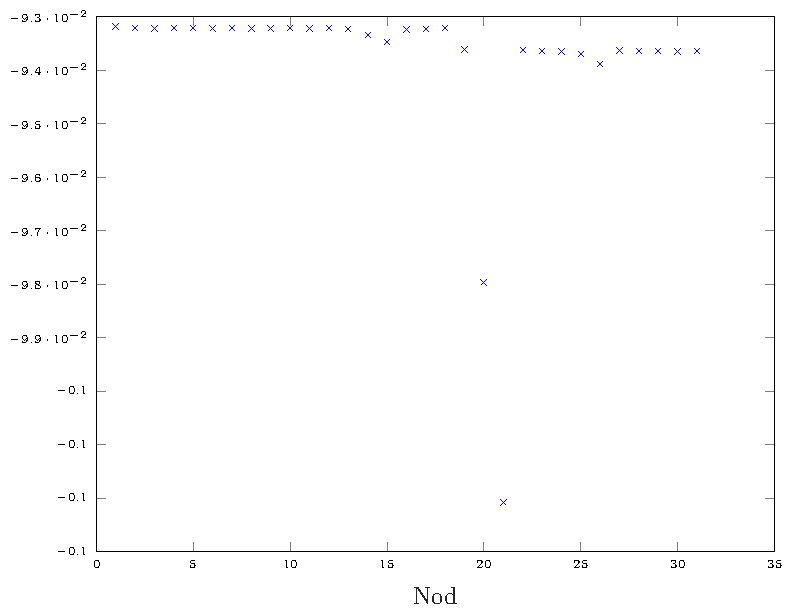
\includegraphics[width=0.5\textwidth]{\pics/c3_pics/residuals/atem_res_emitter21_mag25}%
  \label{fig:residual_atemp_21}%
}&

\subfloat[Reziduuri pentru defect în nodul 27, magnitudine 25]{%
  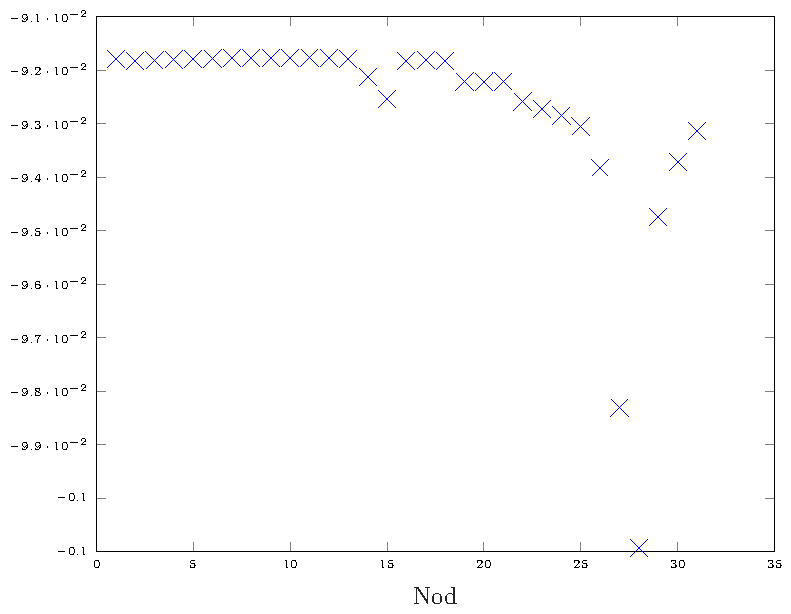
\includegraphics[width=0.5\textwidth]{\pics/c3_pics/residuals/atem_res_emitter27_mag25}%
  \label{fig:residual_atemp_27}%
} 
\end{tabular}
\caption{Reziduuri atemporale rețea}
\label{fig:rez_atemp}
\end{figure}

Asemenea reziduurilor de la \ref{fig:rez_time} se poate observa că simularea unui emitter într-un nod va determina un răspuns puternic în nodul respectiv și în vecinătatea nodului afectat